\section{Machine-learning methodology}
\label{sec:methodology}
% =============================================================================

\subsection{Overview and comparison principle}
\label{subsec:methodology_overview}

The models in this work approximate two related but distinct operators. The longitudinal branch acts directly on a one-dimensional density, whereas the six-dimensional branch acts on the reduced representation defined in Eq.~\eqref{eq:histogram_representation_revised}. For a dataset
\begin{equation}
    \mathcal{D}
    =
    \left\{
        \left(a^{(s)},\mu^{(s)},u^{(s)}\right)
    \right\}_{s=1}^{N},
\end{equation}
the general training objective is
\begin{equation}
    \theta^{\star}
    =
    \operatorname*{arg\,min}_{\theta}
    \frac{1}{N}
    \sum_{s=1}^{N}
    \ell\!\left(
        \mathcal{G}_{\theta}(a^{(s)},\mu^{(s)}),
        u^{(s)}
    \right).
    \label{eq:operator_training_revised}
\end{equation}
The choice of representation and interaction support, rather than generic neural-network depth alone, distinguishes the models compared below.

\begin{figure}[H]
    \centering
    \resizebox{0.96\textwidth}{!}{%
    \begin{tikzpicture}[
        node distance=1.15cm and 1.35cm,
        box/.style={draw,rounded corners,align=center,minimum width=3.2cm,minimum height=0.9cm},
        arrow/.style={-{Latex[length=2.5mm]},thick}
    ]
        \node[box] (sim) {Simulation data\\particle clouds and parameters};
        \node[box,below left=of sim] (long) {Longitudinal profile\\$\lambda_{\mathrm{in}}$};
        \node[box,below right=of sim] (pair) {Pairwise representation\\$\mathcal{H}(\rho),\bm m,\bm\sigma$};
        \node[box,below=of long] (fno) {Fourier Neural Operator};
        \node[box,below=of pair] (cvae) {CVAE encoder\\$q_{\phi}(z\mid\mathcal{H},\bm m,\bm\sigma,d)$};
        \node[box,below=of cvae] (prop) {Global Transformer / Windowed Transformer / GNO};
        \node[box,below left=of prop] (dec) {Histogram decoder\\$\widehat{\mathcal{H}}(\rho_N)$};
        \node[box,below right=of prop] (phys) {Physical-statistics head\\$\widehat{\bm m}_N,\widehat{\bm\sigma}_N$};
        \node[box,below=of fno] (lout) {Predicted profile\\$\widehat{\lambda}_{\mathrm{out}}$};
        \draw[arrow] (sim) -- (long);
        \draw[arrow] (sim) -- (pair);
        \draw[arrow] (long) -- (fno);
        \draw[arrow] (fno) -- (lout);
        \draw[arrow] (pair) -- (cvae);
        \draw[arrow] (cvae) -- (prop);
        \draw[arrow] (prop) -- (dec);
        \draw[arrow] (prop) -- (phys);
    \end{tikzpicture}}
    \caption{Implemented modelling hierarchy. The FNO acts on reduced longitudinal profiles. The CVAE compresses the fifteen pairwise marginals; three alternative propagators then evolve the same latent representation. A decoder reconstructs projected density shape, while a separate head predicts six centroids and six RMS sizes.}
    \label{fig:ml_architecture_overview}
\end{figure}

The comparison between latent propagators uses the same trajectory split, histogram preprocessing, coordinate order, CVAE representation, and output targets. This design reduces, but does not eliminate, confounding from optimisation and random initialisation. The reported comparison corresponds to one selected checkpoint per configuration; repeated-seed uncertainty is therefore identified as a limitation rather than inferred from test-sample variation.

\subsection{Fourier Neural Operator}
\label{subsec:fourier_neural_operator}

The longitudinal problem is a map between functions sampled on the same uniform grid,
\begin{equation}
    \widehat{\mathcal{T}}_{\theta}:
    (\lambda_{\mathrm{in}},\mu)
    \longmapsto
    \widehat{\lambda}_{\mathrm{out}}.
    \label{eq:fno_main_task}
\end{equation}
For a hidden field $v_{\ell}(z)$, one FNO layer is
\begin{equation}
    v_{\ell+1}(z)
    =
    \sigma\!\left[
        W_{\ell}v_{\ell}(z)
        +
        \mathcal{F}^{-1}
        \left(
            R_{\theta,\ell}(k)\mathcal{F}[v_{\ell}](k)
        \right)(z)
        +b_{\ell}(z)
    \right],
    \label{eq:fno_layer_revised}
\end{equation}
where only a finite set of Fourier modes is retained. The spectral parameterisation is compatible with the convolutional structure of wakefields,
\begin{equation}
    V_{\mathrm{ind}}(z)
    =
    -\mathcal{F}^{-1}
    \left[
        Z_{\parallel}(\omega)\widehat{\lambda}(\omega)
    \right](z),
\end{equation}
but the learned multiplier $R_{\theta,\ell}$ is not interpreted as the physical impedance. It approximates the complete transformation represented in the training data, including RF confinement, relaxation, parameter dependence, and discretisation effects. The study does not experimentally test cross-resolution transfer; the FNO is evaluated on the grid used for training.

\subsection{Conditional variational representation}
\label{subsec:variational_latent_representation}

\subsubsection{Inputs and conditioning}

The CVAE input is the complete channel tensor
\begin{equation}
    X=\mathcal{H}(\rho)\in\mathbb{R}^{15\times64\times64}.
\end{equation}
The explicit physical vector contains six coordinate centroids and six RMS sizes in the data order of Eq.~\eqref{eq:data_coordinate_order},
\begin{equation}
    a
    =
    [\bm\sigma,\bm m]
    \in
    \mathbb{R}^{12}.
\end{equation}
A two-component domain indicator distinguishes input and output snapshots,
\begin{equation}
    d_{\mathrm{in}}=(1,0),
    \qquad
    d_{\mathrm{out}}=(0,1).
\end{equation}
The domain indicator contains no target value; it only identifies which of the two snapshot domains is being reconstructed. Splitting by trajectory before concatenation prevents it from coupling train and test states.

\subsubsection{Encoder, posterior, and decoder}

Four residual convolutional blocks map
\begin{equation}
    15\times64\times64
    \longrightarrow
    32\times32\times32
    \longrightarrow
    64\times16\times16
    \longrightarrow
    128\times8\times8
    \longrightarrow
    256\times4\times4.
    \label{eq:cvae_encoder_shapes}
\end{equation}
After flattening, the 4096 convolutional features are concatenated with $a$ and $d$ and projected to $h\in\mathbb{R}^{1024}$. Two heads parameterise a diagonal Gaussian posterior,
\begin{equation}
    q_{\phi}(z\mid X,a,d)
    =
    \mathcal{N}\!\left(
        \bm\mu_z,
        \operatorname{diag}(\bm\sigma_z^2)
    \right),
    \qquad
    z\in\mathbb{R}^{512},
    \label{eq:cvae_posterior}
\end{equation}
with
\begin{equation}
    z
    =
    \bm\mu_z
    +
    \bm\sigma_z\odot\epsilon,
    \qquad
    \epsilon\sim\mathcal{N}(0,I).
    \label{eq:cvae_reparameterisation}
\end{equation}

The decoder receives $(z,d)$, but not $a$. It reconstructs normalised pairwise morphology through four residual upsampling blocks and a final $1\times1$ convolution. Therefore, the report does not claim that physical scale is supplied directly to the decoder. Instead, scale and position are supervised explicitly through the physical-statistics branch and may also be represented implicitly in $z$ because the encoder used $a$. This asymmetric conditioning is important when interpreting the latent-correlation diagnostic.

For channel $p$, non-negativity and unit mass are imposed by
\begin{equation}
    \widetilde{H}_p
    =
    \operatorname{ReLU}(G_p),
    \qquad
    \widehat{H}_p(u,v)
    =
    \frac{\widetilde{H}_p(u,v)}
    {\sum_{u',v'}\widetilde{H}_p(u',v')+\varepsilon}.
    \label{eq:cvae_channel_normalisation}
\end{equation}
If the denominator is numerically negligible, a uniform channel is used to avoid division by zero. Unit-mass normalisation enforces mass conservation for each projected probability map, but it does not enforce consistency among channels sharing one coordinate.

\subsubsection{Snapshot-pretraining objective}

Initial and final snapshots from training trajectories are concatenated only after the split. The implemented loss is
\begin{equation}
    \mathcal{L}_{\mathrm{CVAE}}
    =
    \mathcal{L}_{\mathrm{rec}}^{\mathrm{in}}
    +
    \mathcal{L}_{\mathrm{rec}}^{\mathrm{out}}
    +
    \beta\mathcal{L}_{\mathrm{KL}}
    +
    \gamma\mathcal{L}_{\sigma}
    +
    \delta\mathcal{L}_{m},
    \label{eq:cvae_complete_loss}
\end{equation}
with $\beta=10^{-2}$ and $\gamma=\delta=10^{-3}$. The KL term is
\begin{equation}
    \mathcal{L}_{\mathrm{KL}}
    =
    \frac{1}{2}
    \mathbb{E}
    \left[
        \sum_{j=1}^{512}
        \left(
            \mu_{z,j}^{2}
            +\sigma_{z,j}^{2}
            -1
            -\log\sigma_{z,j}^{2}
        \right)
    \right].
    \label{eq:cvae_kl_loss}
\end{equation}
RMS sizes are supervised in logarithmic space to preserve positivity and balance scales,
\begin{equation}
    \mathcal{L}_{\sigma}
    =
    \operatorname{MSE}
    \left(
        \log\widehat{\bm\sigma},
        \log\bm\sigma
    \right),
\end{equation}
while $\mathcal{L}_m=\operatorname{MSE}(\widehat{\bm m},\bm m)$. Reported KL values are given both as totals and per latent coordinate because the total grows with $d_z$; only the weighted contribution $\beta\mathcal{L}_{\mathrm{KL}}$ enters the optimisation objective.

\subsection{Tokenised latent dynamics}
\label{subsec:tokenized_latent_dynamics}

The pretrained encoder maps the initial state to $z_0$. A propagator then predicts a residual latent evolution conditioned on the ordered lattice tokens,
\begin{equation}
    z_{i+1}
    =
    z_i+\Delta z_i,
    \qquad
    \Delta z_i=f_{\theta}(z_i,h_i,\mu),
    \label{eq:latent_propagator_revised}
\end{equation}
where $h_i$ includes element type, length, continuous position, local element parameters, and global conditioning variables. Continuous position is expanded using Fourier features so that the model can represent several longitudinal scales.

\subsubsection{Global causal Transformer}

For token embeddings $H\in\mathbb{R}^{N\times d}$, one attention head is
\begin{equation}
    \operatorname{Attn}(Q,K,V)
    =
    \operatorname{softmax}
    \left(
        \frac{QK^{\top}}{\sqrt{d_k}}
        +M
    \right)V.
    \label{eq:attention_revised}
\end{equation}
The global causal mask permits keys $j\leq i$ and excludes future positions. It therefore preserves directionality but allows direct interaction with the complete upstream sequence \cite{vaswani_attention_2017}.

\subsubsection{Finite-window causal Transformer}

The symbol $W$ denotes the number of accessible tokens, including the current token. The mask is
\begin{equation}
    M_{ij}^{(W)}
    =
    \begin{cases}
        0,
        & \max(1,i-W+1)\leq j\leq i,\\
        -\infty,
        & \text{otherwise}.
    \end{cases}
    \label{eq:window_mask_revised}
\end{equation}
Thus, $W=1$ is self-only attention and $W=4$ gives the four-token band illustrated in Fig.~\ref{fig:causal_window_masks}. The hidden dimension, heads, feed-forward width, and output projection remain unchanged; the window modifies graph connectivity rather than merely reducing network size. After $L$ layers, information can propagate indirectly over at most approximately $1+L(W-1)$ upstream positions in the absence of a global bypass.

\begin{figure}[H]
    \centering
    \resizebox{0.83\textwidth}{!}{%
    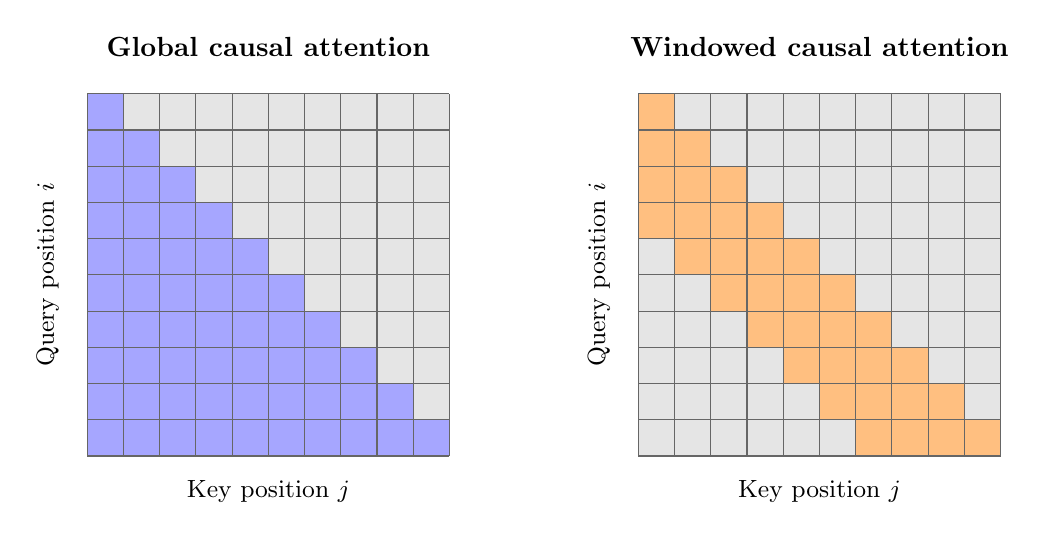
\begin{tikzpicture}[font=\small]
        \def\c{0.46}
        \foreach \panel/\shift/\kind in {Global/0/0,Windowed/7/1}{
            \begin{scope}[xshift=\shift cm]
                \node[font=\bfseries] at (2.3,5.2) {\panel\ causal attention};
                \foreach \i in {1,...,10}{
                    \pgfmathtruncatemacro{\lo}{max(1,\i-3)}
                    \foreach \j in {1,...,10}{
                        \pgfmathsetmacro{\x}{(\j-1)*\c}
                        \pgfmathsetmacro{\y}{(10-\i)*\c}
                        \ifnum\j>\i
                            \fill[gray!20] (\x,\y) rectangle ++(\c,\c);
                        \else
                            \ifnum\kind=1
                                \ifnum\j<\lo
                                    \fill[gray!20] (\x,\y) rectangle ++(\c,\c);
                                \else
                                    \fill[orange!50] (\x,\y) rectangle ++(\c,\c);
                                \fi
                            \else
                                \fill[blue!35] (\x,\y) rectangle ++(\c,\c);
                            \fi
                        \fi
                    }
                }
                \draw[step=\c,black!60,thin] (0,0) grid (4.6,4.6);
                \node at (2.3,-0.45) {Key position $j$};
                \node[rotate=90] at (-0.5,2.3) {Query position $i$};
            \end{scope}
        }
    \end{tikzpicture}}
    \caption{Support of global causal attention and a four-token causal window. Grey entries are masked. The current token is included in $W$.}
    \label{fig:causal_window_masks}
\end{figure}

\subsubsection{Graph Neural Operator}
\label{subsec:graph_neural_operator}

The lattice is represented as a directed graph $\mathcal{G}=(\mathcal{V},\mathcal{E})$. Nodes correspond to lattice elements or observation positions and incoming edges define the admissible upstream neighbourhood $\mathcal{N}_{G}(i)$. A latent GNO layer is
\begin{equation}
    v_i^{(\ell+1)}
    =
    \sigma\!\left[
        W_{\ell}v_i^{(\ell)}
        +
        \sum_{j\in\mathcal{N}_{G}(i)}
        \omega_{ij}
        K_{\theta,\ell}
        \left(h_i,h_j,v_i^{(\ell)},v_j^{(\ell)},\mu\right)
        v_j^{(\ell)}
    \right].
    \label{eq:gno_message_passing_revised}
\end{equation}
The implemented kernel receives relative position and element features; four graph-operator layers are used in the reported GNO. The kernel is an effective interaction in latent space and is not identified with a physical wake, transfer matrix, or Green function.

At the non-local interaction level, both windowed attention and the GNO have the discrete form
\begin{equation}
    (\mathcal{K}_{\Theta}v)_i
    =
    \sum_{j=1}^{N}
    A_{ij}K_{\Theta}(i,j,v_i,v_j,\mu)v_j.
    \label{eq:common_discrete_kernel}
\end{equation}
For attention, $A_{ij}$ is the causal band and $K_{\Theta}$ is softmax-normalised query--key compatibility. For the GNO, $A_{ij}$ is the directed graph adjacency and $K_{\Theta}$ is an explicitly parameterised graph kernel. This is a computational correspondence, not a proof that the physical dynamics have compact support.

\subsection{Physical-statistics head}
\label{subsec:physical_statistics_head}

The histogram decoder predicts normalised distributional shape. A separate head predicts the absolute six-dimensional centroids and RMS sizes,
\begin{equation}
    (z_N,\bm m_0,\log\bm\sigma_0,\mu)
    \longmapsto
    (\widehat{\bm m}_N,\log\widehat{\bm\sigma}_N).
    \label{eq:physical_head_mapping}
\end{equation}
The output has twelve components, not fifteen pair-specific statistics. Pair-specific axes are reconstructed from these six shared coordinate descriptors, which avoids predicting contradictory copies of the same coordinate scale. The head is evaluated independently from the histogram decoder because good normalised shape does not guarantee correct physical position or extension.

\subsection{Losses and validation metrics}
\label{subsec:losses_metrics}

For a test set of $N_{\mathrm{test}}$ paired trajectories and fifteen channels, the mean relative histogram error is
\begin{equation}
    \epsilon_{\mathrm{rel}}
    =
    \frac{1}{15N_{\mathrm{test}}}
    \sum_{s=1}^{N_{\mathrm{test}}}
    \sum_{p=0}^{14}
    \frac{
        \left\|\widehat{H}_{p}^{(s)}-H_{p}^{(s)}\right\|_2
    }{
        \left\|H_{p}^{(s)}\right\|_2+\varepsilon
    }.
    \label{eq:relative_histogram_metric}
\end{equation}
Residual bias is computed on the same normalised maps,
\begin{equation}
    B_H
    =
    \left\|
        \frac{1}{15N_{\mathrm{test}}}
        \sum_{s,p}
        \left(\widehat{H}_{p}^{(s)}-H_{p}^{(s)}\right)
    \right\|_2.
    \label{eq:histogram_bias_metric}
\end{equation}
The Wasserstein-1 distance $W_1$ and sliced-Wasserstein distance $SW$ are reported separately; they are not interchangeable. Physical-statistics errors are
\begin{align}
    \operatorname{MAE}_{m}
    &=
    \frac{1}{6N_{\mathrm{test}}}
    \sum_{s,d}
    \left|\widehat{m}_{d}^{(s)}-m_{d}^{(s)}\right|,
    \\
    \operatorname{MAE}_{\sigma}
    &=
    \frac{1}{6N_{\mathrm{test}}}
    \sum_{s,d}
    \left|\widehat{\sigma}_{d}^{(s)}-\sigma_{d}^{(s)}\right|.
\end{align}
For each coordinate, the coefficient of determination is
\begin{equation}
    R_d^2
    =
    1-
    \frac{
        \sum_s(\widehat{q}_{d}^{(s)}-q_{d}^{(s)})^2
    }{
        \sum_s(q_{d}^{(s)}-\overline{q}_d)^2
    },
    \qquad
    q\in\{m,\sigma\}.
    \label{eq:physics_r2_metric}
\end{equation}
Because most histogram bins are close to zero, $R^2$ is not used as the primary density-map metric; it is reserved for the physical-statistics head. Shared-marginal consistency is evaluated with Eq.~\eqref{eq:marginal_consistency_metric} when the required channel reductions are available.

\begin{table}[H]
    \centering
    \caption{Definitions and scope of the principal validation metrics.}
    \label{tab:metrics_definitions}
    \begin{tabular}{lll}
        \toprule
        Metric & Symbol & Scope \\
        \midrule
        Relative histogram error & $\epsilon_{\mathrm{rel}}$ & Mean over test samples and 15 channels \\
        Wasserstein-1 & $W_1$ & Physical displacement on a projected plane \\
        Sliced Wasserstein & $SW$ & Transport discrepancy from sampled projections \\
        Residual bias norm & $B_H$ & Norm of the mean signed map residual \\
        Centroid/RMS MAE & $\operatorname{MAE}_{m},\operatorname{MAE}_{\sigma}$ & Mean over six coordinates \\
        Coordinate score & $R_d^2$ & Physical-statistics head only \\
        Marginal consistency & $\mathcal{E}_{\mathrm{cons}}$ & Agreement among channels sharing a coordinate \\
        Inference time & $t_{\mathrm{inf}}$ & Neural-model comparison on common hardware \\
        \bottomrule
    \end{tabular}
\end{table}

Inference timing excludes simulation and data generation. A controlled simulator speed-up is therefore not reported. The absence of repeated training seeds, parameter-count matching, and a fixed-$\beta_{\mathrm{KL}}$ window ablation is retained explicitly when interpreting the results.

% =============================================================================
